\documentclass[xetex,mathserif,serif]{beamer}

\begin{document}

\title[Crisis] % (optional, only for long titles)
{On-line summarisation of time-series documents}

\author % (optional, for multiple authors)
{Ersi~Ni}
\institute[University College Dublin] % (optional)
{
	Supervisor: Dr. Dong, Prof. Dr. Smyth \\
  School of Computer Science\\
  University College Dublin
}
\date % (optional)
{Presentation of FYP, 2017}

\frame{\titlepage}
\begin{frame}
	\frametitle{Agenda}
	\begin{enumerate}
		\item Introduction of the problem
		\item Solution proposal and challenges
		\item Solution stage 1: exploratory analysis on time-series
		\item Solution stage 2: natural language processing
		\item Result with UI Mock-Up
	\end{enumerate}
\end{frame}
\begin{frame}
	\frametitle{A story about hotels (in i.e. Dublin)}
	\begin{enumerate}
		\item User side: Hotel booking

		\item Hotel side: Feedback as reasoning for business decisions

	\end{enumerate}
	

	
%\footnote{
%	My strategy is to engage audience in this slide to introduce the problem in a real scenario. For example:
%	\begin{description}
%		\item How many in the audience have consulted rating and reviews while booking hotels?
%		\item How many in the audience read more than 10 reviews for your interested hotel?
%		\item If you were hotel manager, how would you extract meaning for critics from thousands of reviews?
%	\end{description}
%	}
\end{frame}

\begin{frame}
	\frametitle{Story ctd.}
\begin{enumerate}[*]
	\item Core problem: information overload (reviews)
\end{enumerate}
	For Users:
			\begin{enumerate}
			\item Rating is obvious, but 5 hotels with similar price and similar rating scores, which to choose?
			\item What other users are saying about this hotel?
		\end{enumerate}
	For Hotels:
		\begin{enumerate}
		\item Trending topic (context): Why rating has gone down for the past 3 weeks
		\item Background from the city: Revealing what (periodical) events is happening in the past
		\item Users have chosen us in this August over our competitors because...?
		
		
		\end{enumerate}
		

\end{frame}



\begin{frame}
	\frametitle{Solution Proposal}
	\begin{enumerate}
		\item Using statistics from activities in time periods and rating scores to pin-point representative context.
		\item Summarise the context as information retrieval.
	\end{enumerate}
	
	
\end{frame}

\begin{frame}
	\frametitle{Challenges}
	\begin{enumerate}
		\item Data source 
		\begin{enumerate}
		\item availability
		\item feature set
		\item consistency
		\item technical challenges
		\end{enumerate}
		\item Dimension of the data
		\item Need exploration of the data before asking the real question (Exploratory Analysis)
		\item Text Summarisation (pretty much open topic)
	\end{enumerate}
	
	
	Excerpt of the statistics

\begin{figure}[h]
	\centering
	\fboxsep 2mm
	\begin{tabular}{c|c}
	feature & count \\
	\hline
		word tokens & 17,471,927 \\
		sentences & 1,000,631 \\
		reviews & 200,738 \\
		hotels & 700 (Dublin, Galway and Cork)
	\end{tabular}		
\end{figure}

	
\end{frame}

\begin{frame}
	\frametitle{Data acquisition}
	
\begin{enumerate}
		\item Scrapping from web
		\begin{enumerate}
		\item define feature
		\item parsing
		\item irregularity handling
	\end{enumerate} 
	\item Normalisation and Output:
	\begin{enumerate}
		\item Hotel set [meta data]
		\item Review set [meta data AND review text]
	\end{enumerate}
\end{enumerate}
\end{frame}

\begin{frame}
\frametitle{Exploratory Analysis on time-series}
Hotel is static data consisting of meta data, but reviews are time-series.

\begin{figure}[h]
\centering
\fboxsep 0mm
\begin{tabular}{c|cc}
Top & First & Last\\
\hline
2015-05-26 & 2001-11-28 & 2016-09-19
\end{tabular}
\caption{Timestamp statistics}
\end{figure}

Example exploratory: what can rating scores and count tells us about one hotel for the past 3 years?

This requires further normalisation:

\begin{enumerate}
	\item Subset to 3 years (then by hotel)
	\item And resample to 365 days each year
	\item Aggregation statistics on periods like week, month, 3 months etc.
\end{enumerate}

\end{frame}


\begin{frame}
\frametitle{Exploratory Analysis ctd.}

Gibson Hotel from 2015 to 2016 (subset to 1 year to fit in this slide)

\begin{figure}[h]
\centering
\fboxsep 0mm
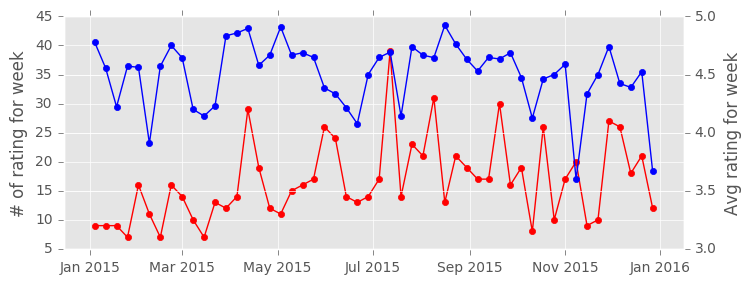
\includegraphics[width=11cm]{gibson_hotel_dublin_rating_score_vs_count}	
\caption{Gibson Hotel aggregated mean rating score and count by week, for 1 year. Red: Count, Blue: average rating score. }
\end{figure}

\end{frame}

\begin{frame}

\frametitle{Stage 2: Text Summarisation}

Assume that we want to investigate the week starting on Sunday the 2015 November 8th for Gibson Hotel.

( the sudden drop in average rating score to mere 3.6 )

We look at the $13$ reviews for Gibson in that week and compare to $869$ reviews for all hotels. 

\begin{tabular}{c}
	\hline
\end{tabular}

Strategy for summarisation:

Construct a $n$ sentences long summary by \textbf{extracting} $n$ \textit{\textbf{key}} sentences from the text pool.


	
\end{frame}

\begin{frame}
	\frametitle{Graph based summarisation}
	\textbf{\textit{Key}} sentences are defined by prestige (importance, uniqueness)
	\begin{enumerate}
		\item Word centrality is defined by a score called $tf\times idf$. 
		\item Sentences are presented as graph notes. Degrees between the notes are voted on a similarity score from a modified formula based on the said centrality.
		\item More connections between notes means more prestige. 
	\end{enumerate}
	
	
	Inspired by Google's Pagerank algorithm, this lexicon modified version called \textbf{LexRank} is introduced by [Erkan \& Radev 2004].
\end{frame}

\begin{frame}
	\frametitle{Visualise the effect of $tf\times idf$ on words.}
\begin{figure}[h]
\centering
\fboxsep 0mm
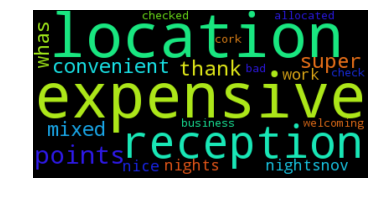
\includegraphics[width=5.2cm]{all_2015_11_08_week}
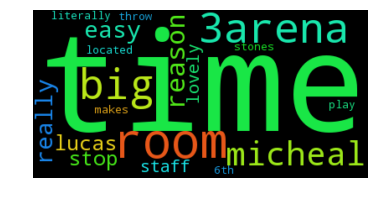
\includegraphics[width=5.2cm]{gibson_2015_11_08_week}

\caption{Word Cloud constructed based on $tf\times idf$ of the reviews for  Dublin (left) and Gibson Hotel (right) in the week from 2015-11-08 to 2015-11-15}

\end{figure}

\end{frame}


\begin{frame}
	\frametitle{Result summarisation with UI Mock-Up}
	\begin{figure}[h]
	\centering
	\fboxsep 0mm
	
	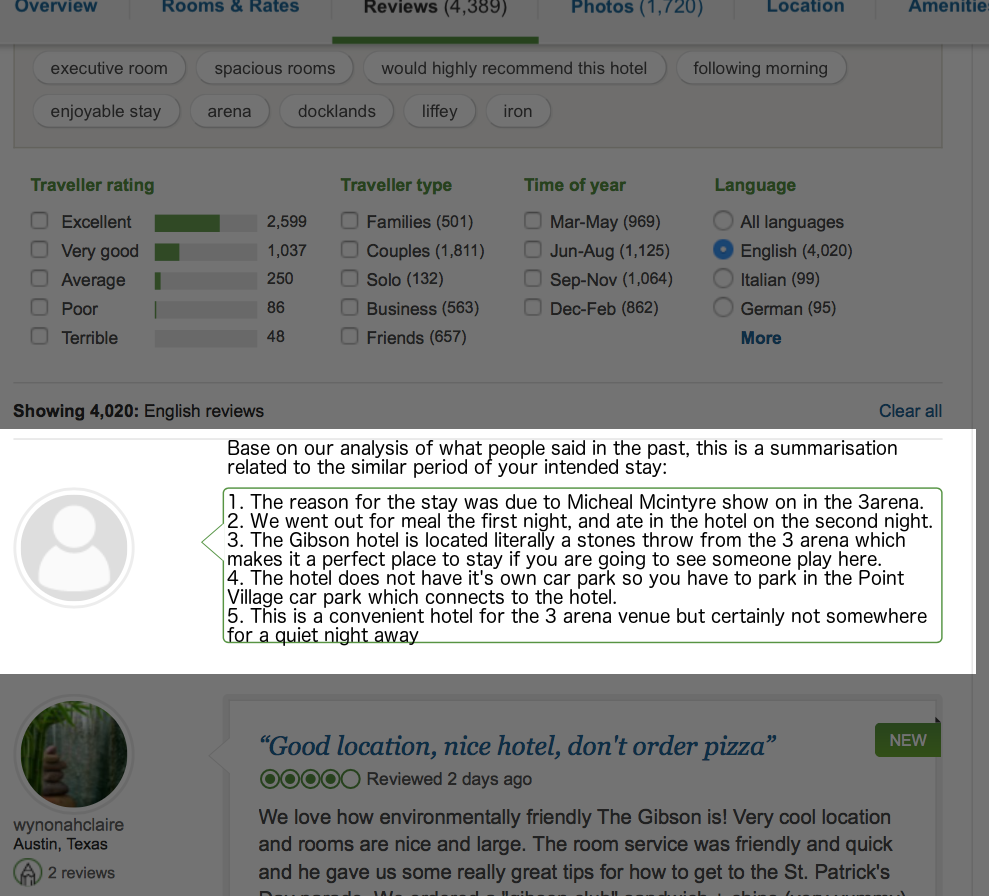
\includegraphics[width=10cm]{ts-3}

	\end{figure}
\end{frame}

\begin{frame}
	\frametitle{Achieved outcome recap}
\begin{enumerate}
		\item Software Pipeline
	\begin{enumerate}
		\item Data acquisition
		\item Software module for time-series manipulation
		\item Software implementation of NLP modules for Graph-based solution
		\item Software implementation for \textbf{LexRank} specifically for multi-document summarisation (different to existing modules available online)
	\end{enumerate}
	
	\item Dataset for future research
	\begin{enumerate}
		\item Hotel and Review meta data as \textbf{csv} files
		\item Raw review text for NLP as compressed archive
		\item Genre (Hotel reviews) wide dataset for NLP [tokens, sentences, term-frequency, inverse-document-frequency etc.]

	\end{enumerate}
	
\end{enumerate}
\end{frame}
\begin{frame}
	\frametitle{Outcome vs original project spec}
	Difference
	\begin{enumerate}
	\item Hotel review as target domain instead of international news
	\item Produced dataset for future research
	\end{enumerate}
	Matched
	\begin{enumerate}
	\item Novelty through combining event detection with existing NLP summarisation
	\item "Live" data summarisation is achievable using cached corpus
	\item Chronology is preserved
	\end{enumerate}
	Pending
	\begin{enumerate}
		\item Evaluation against other time-series summarisation
	\end{enumerate}
\end{frame}




\end{document}
